
\section{Problem definition}

\subsection{Learning a word embedding space}

In order to learn an embedding of words into a vector space, we use the training code provided by Mikolov \etal in word2vec\cite{word2vec}. There are two different models, the Skip-Gram model and the Continuous Bag of words (CBOW) model. Both models consist of a projection layer followed by a softmax layer. They differ in the precise inputs and outputs used. The training data for both models consists of a sequence of words, $w_1, w_2, ..., w_N$. Let $M$ denote the size of the vocabulary (i.e. the number of distinct words in the entire training sequence). We described each of them in turn. 

\subsubsection{Skip Gram}
The Skip-Gram model takes a single word as input and aims to predict the surrounding words, where the order of the surrounding words matters. More specifically, we want to find the parameters $W$ which maximize the conditional log probability of the context of a given word:

\begin{align*}
	\arg \max_{W} \sum_{n=1}^{N} [\sum_{-c \leq t \leq c; t \neq n} \log p(w_{n+c} | w_n; W)]
\end{align*}
where $c$ is the size of the context window being considered (in our experiments we set c = 6). 

The output probability is given by
\begin{align*}
p(w_{O} | w_{I}; W) = \frac{ \exp \big(\phi(w_O) \cdot \phi(w_I) \big)}{\sum_{j=1}^M \exp \big(\phi(w_j) \cdot \phi(w_I) \big)}
\end{align*}


where $\phi(w_i) = W^{\top}x_i$ is the vector representation of $w_i$ (letting $x_i$ denote the 1-hot input vector for with i). The weights $W$ are learned via gradient descent. After training, the final vector representations, $\phi(w_i) \forall i$, are computed front he matrix $W$.



\subsubsection{Continuous Bag of Words (CBOW)}
Unlike the skip gram model, the continuous bag of words makes a bag of words assumption by summing up the projections of the context for a given word and trying to predict the word. More specifically, we want to find the parameters $W$ that maximize the conditional log probability of a word, given the surround words. 
\begin{equation}
	argmax_{\theta} \prod_{w\in text} p(w|k;\theta) \text{ where } k = \sum_{c \in C(w)} v_c
\end{equation}



Given a text corpus, the code provided trains a CBOW or Skip-Gram model and produces a file where every word is assigned a vector in $\mathbb{R}^n$ where we assigned $n=300$.


\begin{figure}[h]
\centering
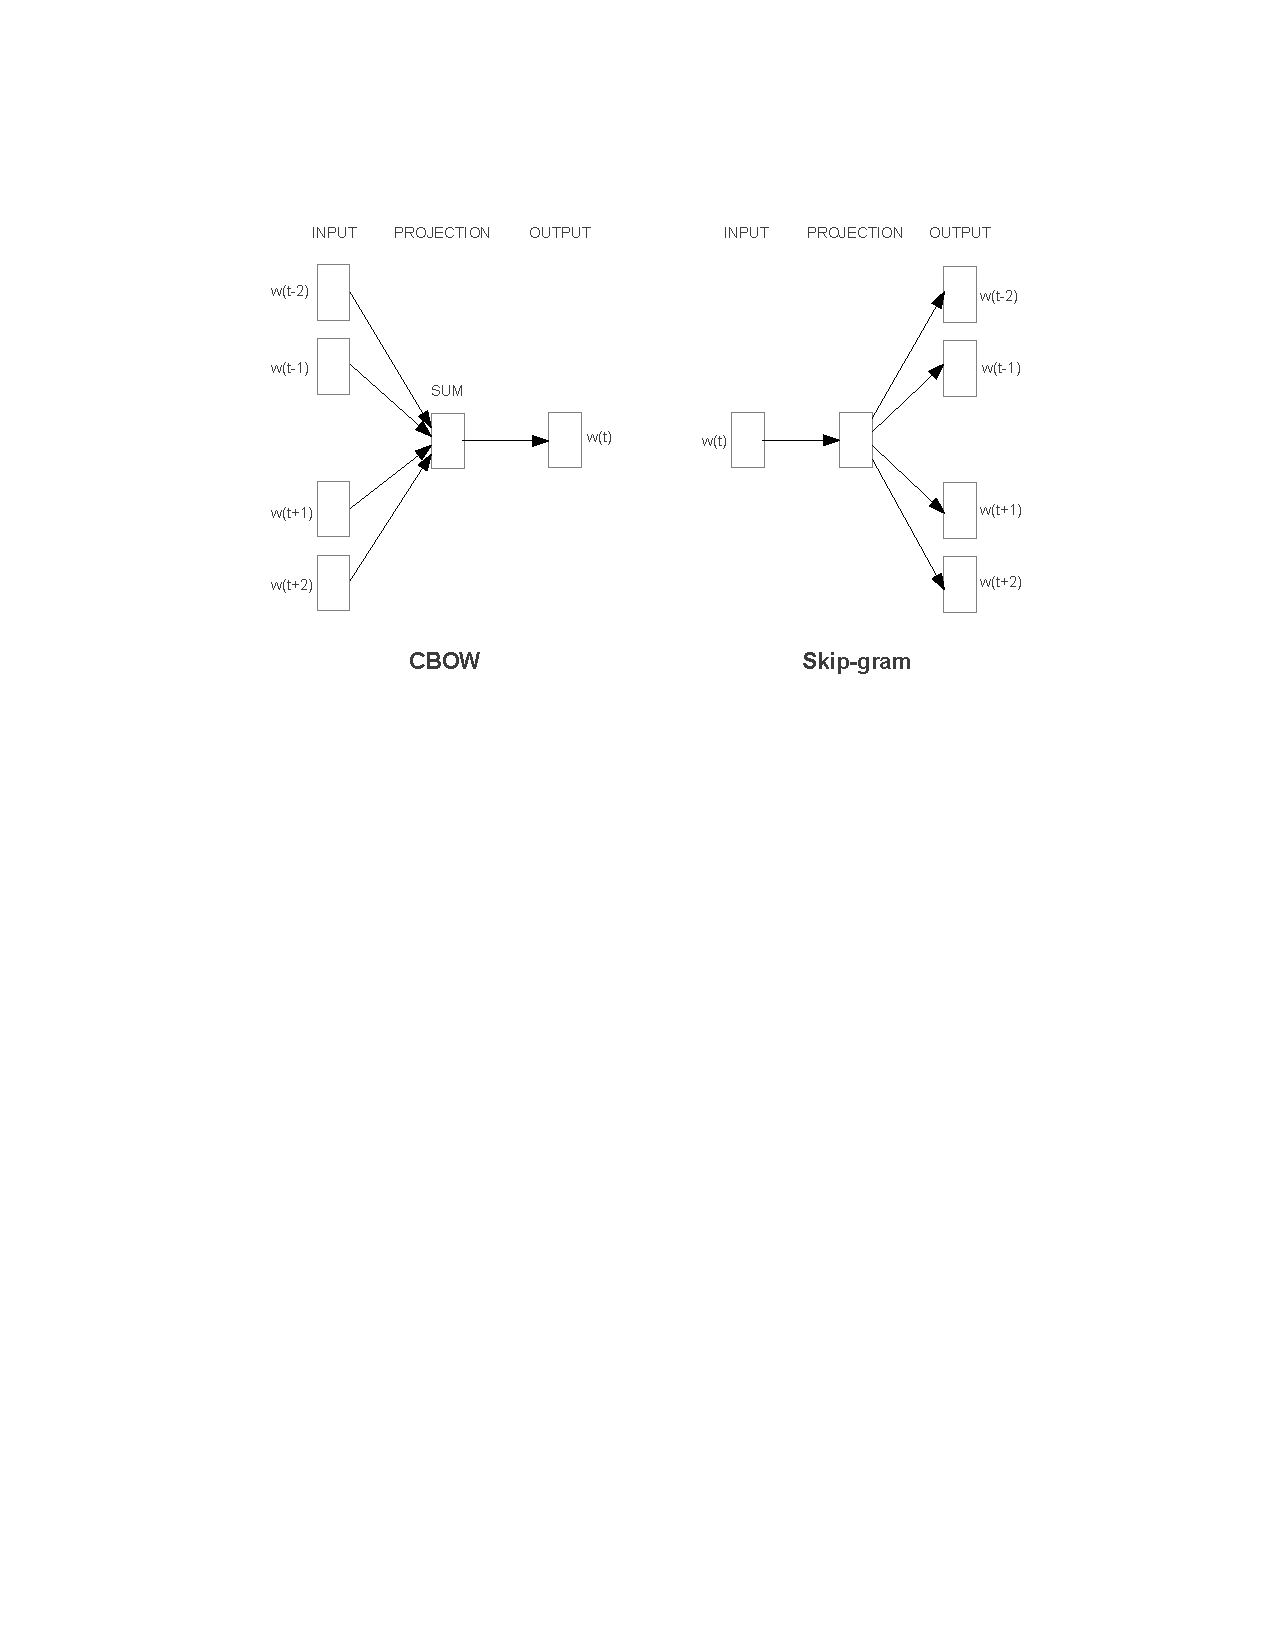
\includegraphics[width=\textwidth]{./images/model_images.pdf}
\caption{CBOW and Skip-Gram Models. Image adopted from \cite{mikolov1}}
\label{fig:top_k}
\end{figure}

\clearpage 


\subsection{Exploring properties of learned word embedding space}